
\documentclass[xcolor={usenames,dvipsnames},12pt,presentation,aspectratio=169]{beamer}

\usepackage[utf8]{inputenc}
\usepackage[brazilian]{babel}
\usepackage{verbatim}
\usepackage{graphicx}
\usepackage{xspace}
\usepackage{amsthm}
\usepackage{url}
\usepackage{array}
\usepackage{hyperref}
\usepackage{times,mathptmx}
\usepackage{pdfpages}
\usepackage{mdframed}
\usepackage{tikz}
\usepackage{alltt}
%\usepackage[usenames,dvipsnames]{xcolor}
%\usepackage[usenames,dvipsnames]{color}
%\usepackage{color}

\usetikzlibrary{arrows,shapes}

\usetheme{Madrid}
%\usetheme{Boadilla}
%\usetheme{Darmstadt}
%\usetheme{Frankfurt}
%\usetheme{CambridgeUS}
%\usetheme{AnnArbor}
%\usecolortheme{beaver}
%\usecolortheme{seahorse}
%\usecolortheme{seagull}
\usecolortheme[named=BrickRed]{structure}

\setbeamercovered{transparent}

\setbeamertemplate{footline}[frame number]
%\setbeamertemplate{navigation symbols}{}
%\setbeamersize{text margin left=1em,text margin right=1em}

\newcommand{\titulo}{Introdução a Programação Paralela}
\newcommand{\disciplina}{ELC139 - Programação Paralela}
\newcommand{\nome}{João Vicente Ferreira Lima (UFSM)}

\lecture[1]{\aula}{aula01}
\def\lecturename{\aula}

\newcommand{\Red}[1]{{\color{red}#1}}
\newcommand{\red}[1]{{\color{red}#1}}
\newcommand{\Blue}[1]{{\color{blue}#1}}
\newcommand{\blue}[1]{{\color{blue}#1}}

\newcommand{\PBS}[1]{\let\temp=\\#1\let\\=\temp}
\newcommand{\RRCOL}{\PBS\raggedright\hspace{0pt}}

\newcommand{\p}[1]{\texttt{#1}}
\newenvironment{code}{%
  \begin{alltt}%
  }{%
  \end{alltt}%
}

\makeatletter
%\setbeamertemplate{headline}{}
% {%
%   \leavevmode%
%   \@tempdimb=2.4375ex%
%   \ifnum\beamer@subsectionmax<\beamer@sectionmax%
%     \multiply\@tempdimb by 4%
%   \else%
%     \multiply\@tempdimb by\beamer@subsectionmax%
%   \fi%
%   \ifdim\@tempdimb>0pt%
%     \advance\@tempdimb by 1.125ex%
%     \begin{beamercolorbox}[wd=.5\paperwidth,ht=\@tempdimb]{section in head/foot}%
%       \vbox to\@tempdimb{\vfil\insertsectionnavigation{.5\paperwidth}\vfil}%
%     \end{beamercolorbox}%
%     \begin{beamercolorbox}[wd=.45\paperwidth,ht=\@tempdimb]{subsection in head/foot}%
%       \vbox
%       to\@tempdimb{\vfil\insertsubsectionnavigation{.45\paperwidth}\vfil}%
%     \end{beamercolorbox}%
%     \begin{beamercolorbox}[wd=.05\paperwidth,ht=\@tempdimb]{subsection in head/foot}%
%       \vbox
%       to\@tempdimb{\vfil\hfil\insertframenumber\vfil\vfil}%
%     \end{beamercolorbox}%
%   \fi%
% }

\def\dohead{\beamer@headcounter=4\relax\beamer@headcounter=1\loop\ifnum\beamer@headcounter<\beamer@totalheads%
  \advance\beamer@headcounter by1\relax%
  \csname @@head\the\beamer@headcounter\endcsname\repeat}

\makeatother

\title[\titulo]{\titulo}

\subtitle{\disciplina}

\author[João V. F. Lima]{\nome}

%\institute[UFSM]{Departamento de Linguagens e Sistemas de Computação \\ Universidade Federal de Santa Maria \\ \url{jvlima@inf.ufsm.br} \\ \url{http://www.inf.ufsm.br/~jvlima}}
\institute[UFSM]{Universidade Federal de Santa Maria \\ \url{jvlima@inf.ufsm.br} \\ \url{http://www.inf.ufsm.br/~jvlima}}
\date{2023/1}

\graphicspath{{.}{figs/}}

\logo{ 
\includegraphics[height=1.5cm,width=1.5cm,keepaspectratio]{logo_inf}    
        
\includegraphics[height=1.5cm,width=1.5cm,keepaspectratio]{logo_ufsm} }

%\titlegraphic{
%	
\includegraphics[width=2cm]{logo_ufsm}
%  \hspace{1cm}
%	
\includegraphics[width=2cm]{logo_inf}
%}

\newtheorem{mydef}{Definição}[section]
%\newtheorem{myteo}{Teorema}[section]
%------------------------------------------------------------------------------
%\newcommand{\xkaapi}{XKaapi\xspace}
%------------------------------------------------------------------------------
% Typesetting Listings
\usepackage{listings}
\lstset{
  language=C++,
  %basicstyle=\scriptsize\ttfamily,
  %basicstyle=\normalsize\ttfamily,
  basicstyle=\small\ttfamily,
  %basicstyle=\footnotesize\ttfamily,
  aboveskip=0pt,
  belowskip=0pt,
  mathescape=false,
  columns=flexible,
  numbers=none,
%  numbers=left,
%  showtabs=true,
%  showspaces=true,
  breaklines=true
}
%------------------------------------------------------------------------------
\lstset{commentstyle=\color{blue}}
%\lstset{stringstyle=\ttfamily}
%\lstset{ classoffset=1, 
%            morekeywords={kaapi,omp,task,data,alloca, declare, reduction, identity, parallel,sync,taskwait,cilk,spawn,tbb,css,cilk\_spawn,cilk\_sync,cilk\_for,offload},
%            keywordstyle=\color{Red}\bfseries
%           }
%\lstset{ classoffset=2, 
%            morekeywords={value,read,write,readwrite,reduction,untied,firstprivate,TaskBodyCPU,TaskBodyGPU,ka,Signature,RW,CW,range2d\_r,range2d\_rw,range2d,Spawn,Fork,Shared\_w,Shared\_r,Shared,a1,target,device,copyin,copyout,input,implements,copy\_deps,RPWP,range2d\_rpwp,rangeindex,Memory,Register,SetStaticSched,Sync,Unregister,Community,System,join\_community,SpawnMain,leave,initialize,terminate,logfile,array,SetArch,ArchHost,ArchCUDA,W,R,gpuStream,pointer\_w,pointer\_r,pointer\_cw,pointer},
%            keywordstyle=\color{Blue}\bfseries
%           }
%\lstset{ classoffset=3, 
%            morekeywords={storage,ld},
%            keywordstyle=\bfseries
%           }
%\lstset{ classoffset=4, 
%            morekeywords={in,out,inout,cout,concurrent},
%            keywordstyle=\color{Red}\bfseries
%           }
%           
\lstset{classoffset=0, showstringspaces=false}
%------------------------------------------------------------------------------
\mdfsetup{
  backgroundcolor=gray!10,
%  roundcorner=10pt,
}
%------------------------------------------------------------------------------
\newcommand{\restorefootline}{\setbeamertemplate{navigation symbols}{}}
%\newcommand{\setfootline}[1]{\setbeamertemplate{navigation symbols}{\textcolor{black}{\textbf{#1}}}}
\newcommand{\includeslides}[4]{%
%  \setfootline{#1}%
  {
    \setbeamercolor{background canvas}{bg=}
    \includepdf[pages={#1},%
    pagecommand={},
%    pagecommand={\begin{frame}[default]{}\end{frame}},
%    #4,%
    turn=false,noautoscale=false,column=false,columnstrict=false,openright=false,frame=false]{#2}%
  }
  %\restorefootline%
}
%------------------------------------------------------------------------------
\begin{document}

\begin{frame}
%  \titlepage
  \maketitle
%  \mode<presentation>
%  {
%    \begin{columns}
%      \begin{column}{0.5\textwidth}
%      \raggedleft
%	
\includegraphics[width=2cm]{logo_ufsm}
%      \end{column}
%      \begin{column}{0.5\textwidth}
%	
\includegraphics[width=2cm]{logo_inf}
%      \end{column}
%    \end{columns}
%  }
\end{frame}

\begin{frame}
    \frametitle{Outline}
    \tableofcontents[hideallsubsections]
%    \tableofcontents
\end{frame}

\AtBeginSection{
  \begin{frame}
    \frametitle{Outline}
    \tableofcontents[currentsection,hideothersubsections]
  \end{frame}
}

%%%%%%%%%%%%%%%%%%%%%%%%%%%%%%%%%%%%%%%%%%%%%%%%%%%%%%%%%%%%%%%%%%%%%%%%%%%%%%
\section{Introdução}
%%%%%%%%%%%%%%%%%%%%%%%%%%%%%%%%%%%%%%%%%%%%%%%%%%%%%%%%%%%%%%%%%%%%%%%%%%%%%%%
%------------------------------------------------------------------------------
\begin{frame}
  \frametitle{Computação Paralela}
    \begin{itemize}
        \item Por que Computação Paralela?
        \item Onde o paralelismo é aplicado?
        \item Primeiro grande motivador: hardware
            \begin{itemize}
                \item Processadores multicore onipresentes
                \item Limites de chip
            \end{itemize}
        \item Segundo: software
            \begin{itemize}
                \item Computação Científica
                \item Data centers e computação em nuvem
            \end{itemize}
    \end{itemize}
\end{frame}
%%%%%%%%%%%%%%%%%%%%%%%%%%%%%%%%%%%%%%%%%%%%%%%%%%%%%%%%%%%%%%%%%%%%%%%%%%%%%%
\section{Hardware}
%%%%%%%%%%%%%%%%%%%%%%%%%%%%%%%%%%%%%%%%%%%%%%%%%%%%%%%%%%%%%%%%%%%%%%%%%%%%%%%
%------------------------------------------------------------------------------
\begin{frame}
  \frametitle{Lei de Moore}
  \vspace{-3mm}
    \begin{columns}
      \begin{column}{0.3\textwidth}
        Gordon Moore (co-fundador da Intel) previu em 1965 que a densidade de transistores
        em chips iria dobrar a cada 18 meses.
     \end{column}
      \begin{column}{0.7\textwidth}
  \begin{center}
	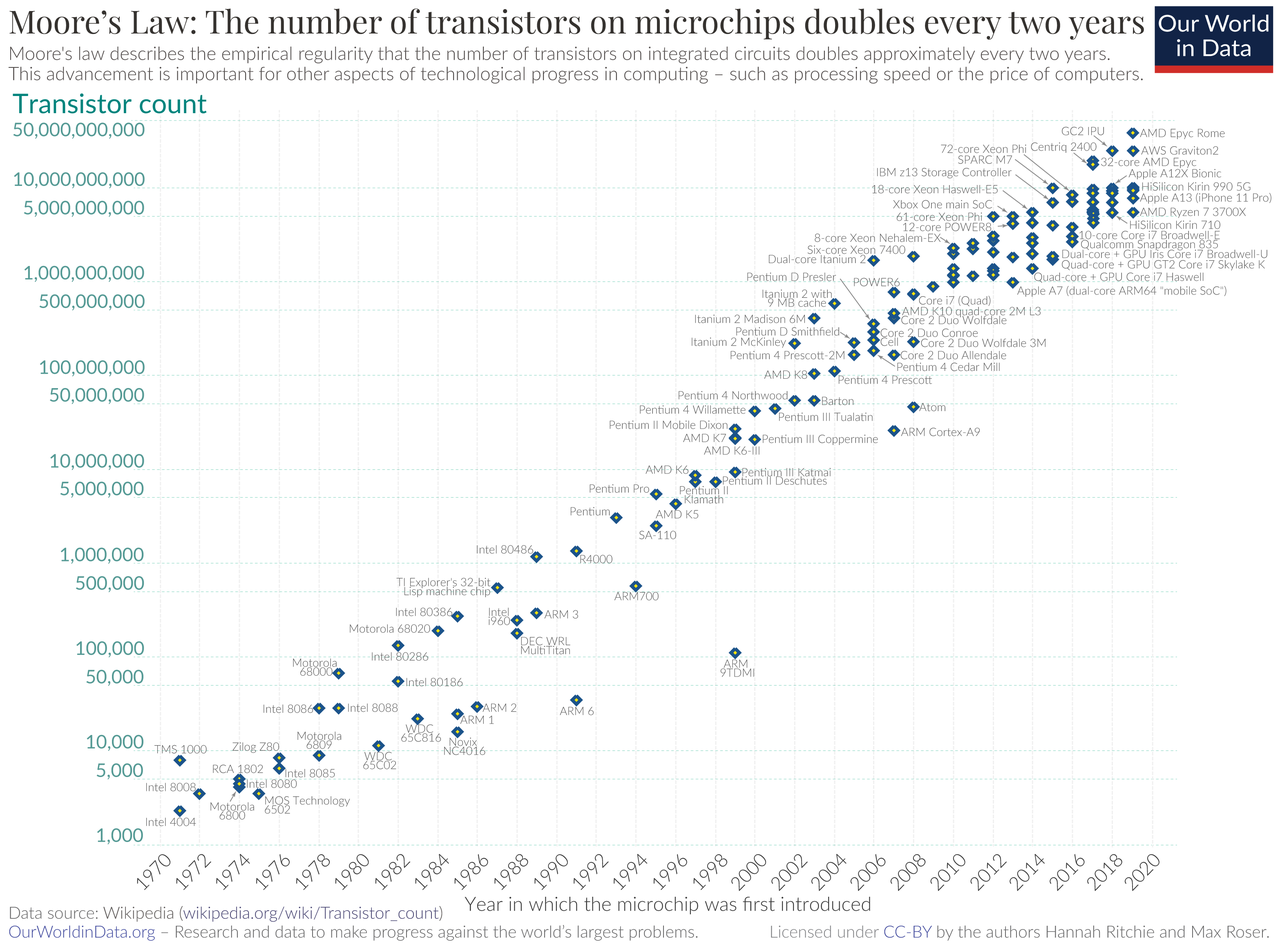
\includegraphics[width=\textwidth]{moore.png}
  \end{center}
      \end{column}
    \end{columns}
\end{frame}
%------------------------------------------------------------------------------
\begin{frame}
  \frametitle{Free Lunch is Over}
  \begin{itemize}
  \item  O clock evoluia de 500 MHz, 1 GHz até 3 GHz 
  \item As CPUs usavam estratégias de ILP para ganho
    \begin{itemize}
        \item Pipeline, superscalar, VLIW (Very Long Instruction Word), SIMD, branch prediction
    \end{itemize}
    \item Ganhos em escala em geral:
    \begin{itemize}
        \item Instruções longas, pipeline profundo
        \item Mais especulação
        \item Mais registradores e cache
    \end{itemize}
    \item Aumenta densidade do chip $\simeq$ aumenta frequência $\simeq$ aumenta desempenho

    \item \textbf{Solução} - sempre comprar um processador novo.
  \end{itemize}
  {\footnotesize \url{https://www.karlrupp.net/2018/02/42-years-of-microprocessor-trend-data/}}
\end{frame}
%------------------------------------------------------------------------------
\begin{frame}
  \frametitle{Evolução dos processadores}
  \vspace{-4mm}
  \begin{center}
	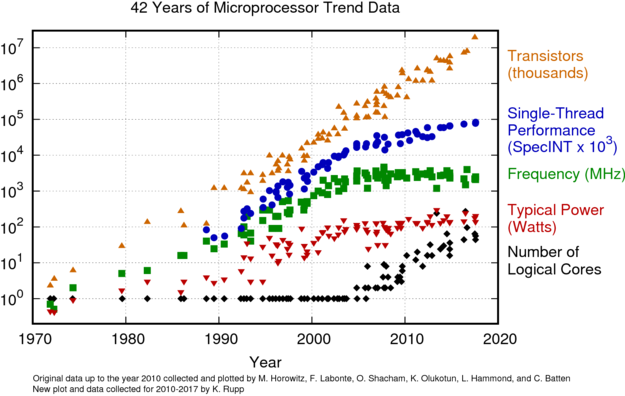
\includegraphics[width=0.7\textwidth]{42-years-processor-trend-625x396.png}
  \end{center}
  {\footnotesize \url{https://www.karlrupp.net/2018/02/42-years-of-microprocessor-trend-data/}}
\end{frame}
%------------------------------------------------------------------------------
\begin{frame}
  \frametitle{Evolução dos processadores}
    \begin{itemize}
      \item Solução é duplicar unidades de processamento no mesmo chip
      \begin{itemize}
        \item Hyperthreading para threads em paralelo
        \item Multicore com uma ou mais CPUs dentro do mesmo chip
      \end{itemize}
      \item 2 x 3 GHz $<$ 6 GHz
      \begin{itemize}
        \item Duas threads no mesmo processador não garatem o dobro de desempenho 
        \item Sobrecusto de coerência de dados
        \item Barramento de memória
        \item Cache compartilhada em grande parte dos casos
      \end{itemize}
    \end{itemize}
  \begin{center}
	%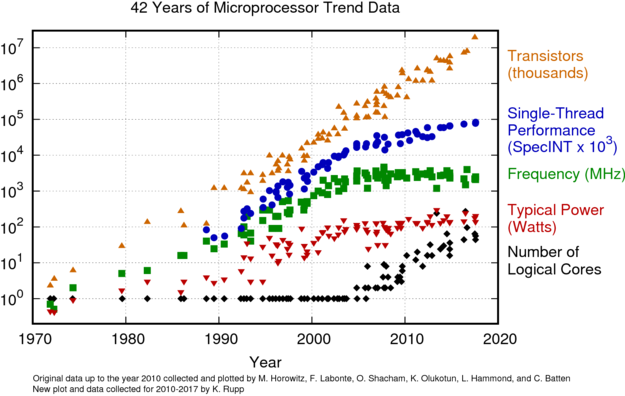
\includegraphics[width=0.7\textwidth]{42-years-processor-trend-625x396.png}
  \end{center}
\end{frame}
%------------------------------------------------------------------------------
%------------------------------------------------------------------------------
%\begin{frame}
%  \frametitle{História do C++}
%    \begin{columns}
%      \begin{column}{0.7\textwidth}
%        \begin{itemize}
%          \item Criado em 1979 como \emph{C with Classes} por Bjarne Stroustrup
%          \item C++ é compatível com C
%          \item Abstrações sem comprometer o desempenho 
%          \item 1985: primeira edição do livro \emph{The C++ Programming Language}
%          \item 1994: STL (\emph{Standard Template Library}) por Alexander Stepanov
%          \item 1998: ISO C++ standard.
%        \end{itemize}
%     \end{column}
%      \begin{column}{0.3\textwidth}
%  \begin{center}
%	
\includegraphics[width=0.8\textwidth]{4thEnglish.jpeg}
%  \end{center}
%      \end{column}
%    \end{columns}
%\end{frame}
%------------------------------------------------------------------------------
% TODO: excessao, etc
%\begin{frame}
%  \frametitle{Entrada e saída}
%  \begin{itemize}
%  \item 
%  \end{itemize}
%\end{frame}
%------------------------------------------------------------------------------
%\begin{frame}
%  \frametitle{Entrada e saída}
%  \begin{itemize}
%  \item 
%  \end{itemize}
%\end{frame}
%------------------------------------------------------------------------------
%------------------------------------------------------------------------------
\begin{frame}
  \frametitle{Data centers}
  \vspace{-3mm}
  \begin{center}
	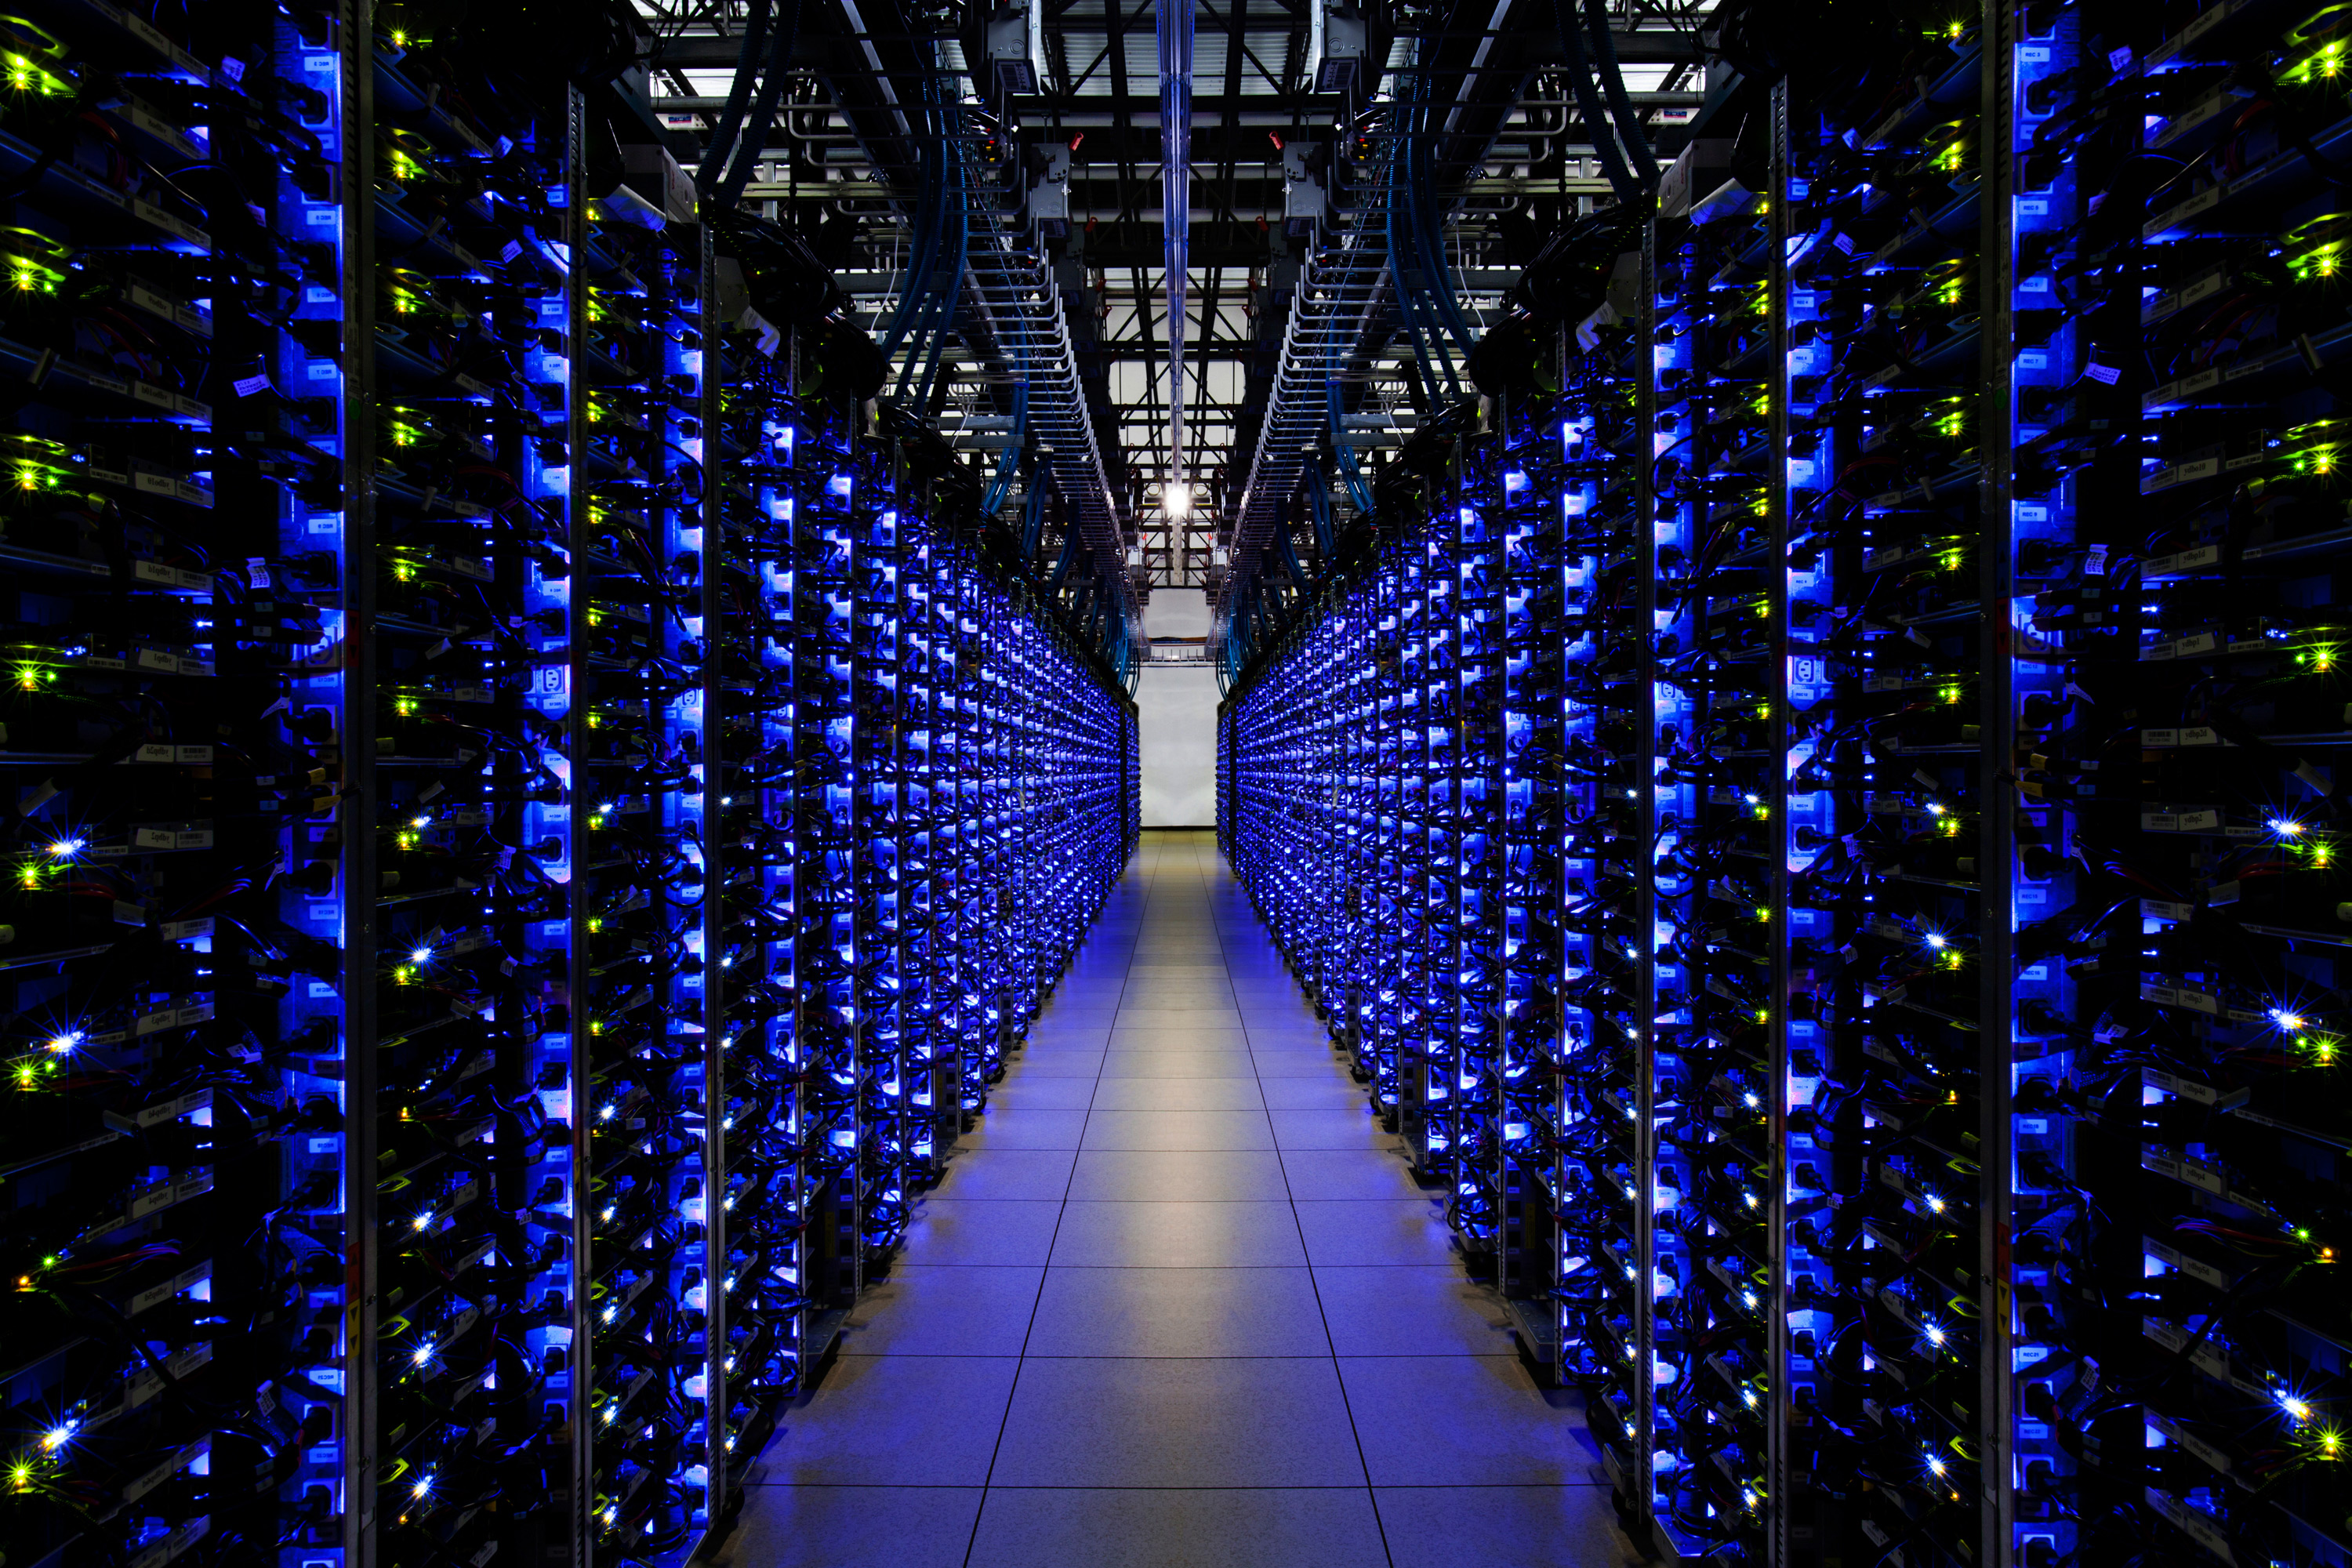
\includegraphics[width=0.7\textwidth]{douglas-county-servers.jpg}
  \end{center}
  {\footnotesize \url{https://www.google.com/intl/pt-BR/about/datacenters/gallery/}}
\end{frame}
%------------------------------------------------------------------------------
\begin{frame}
  \frametitle{Data centers}
  \vspace{-3mm}
  \begin{center}
	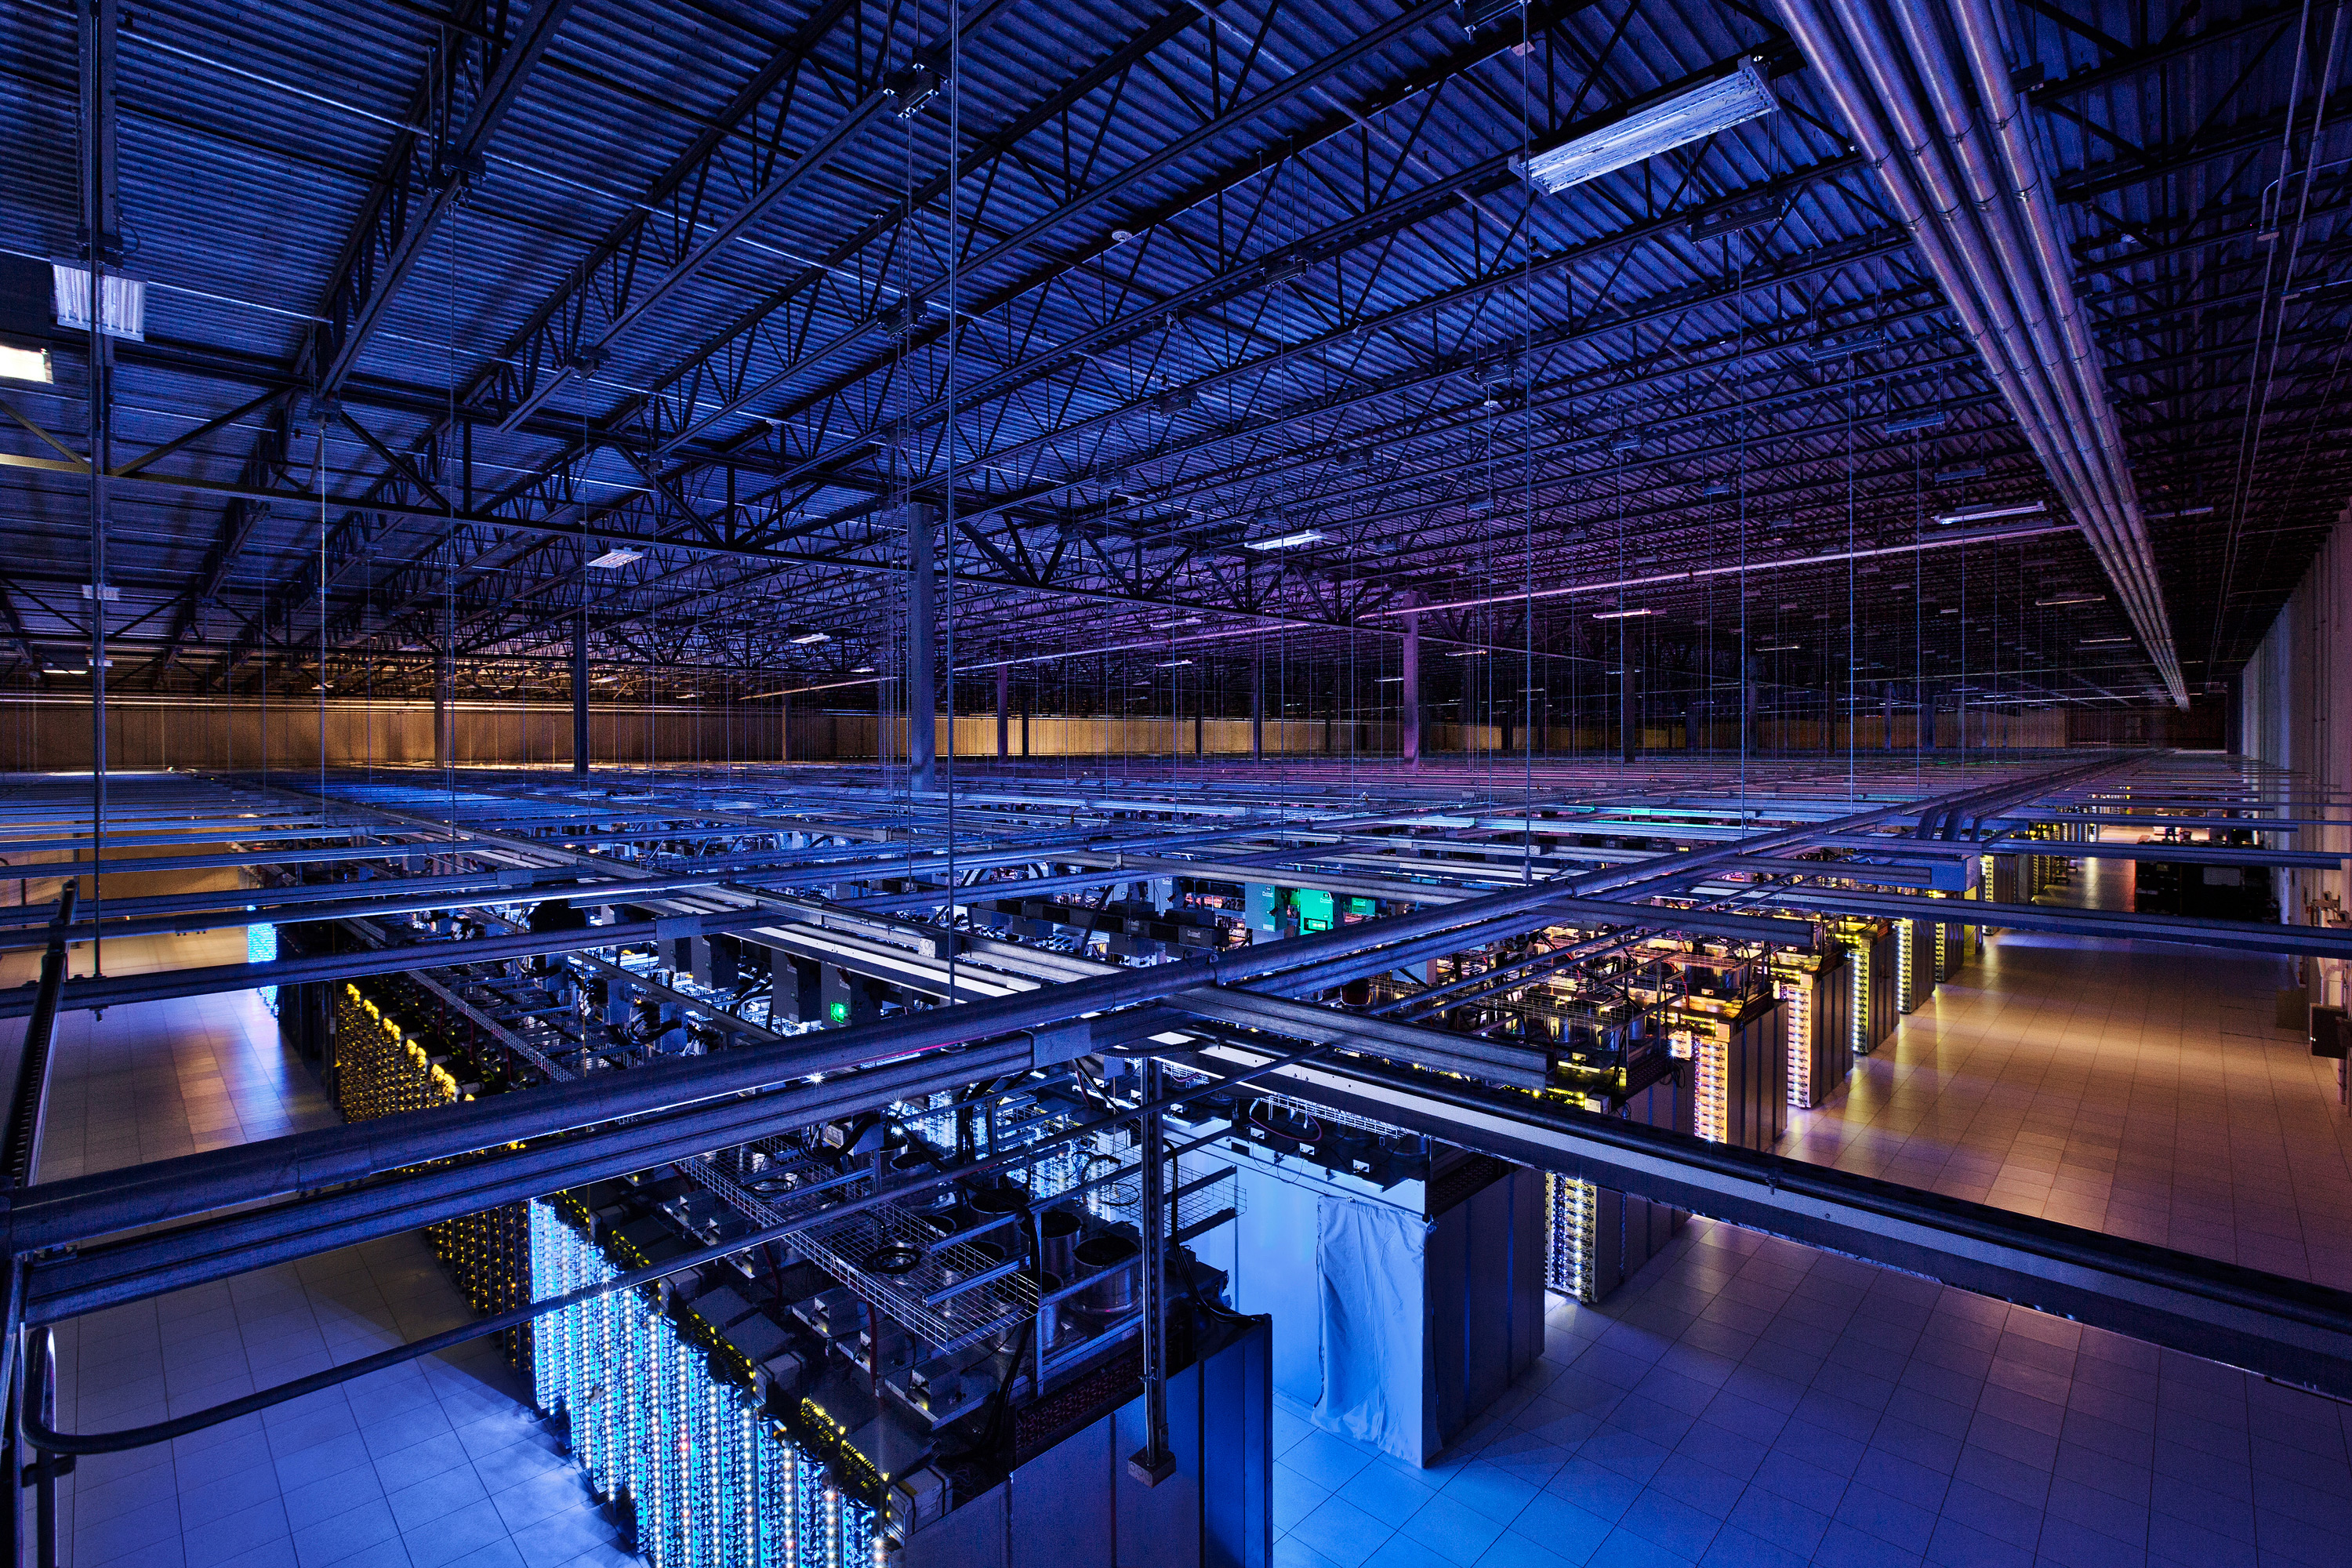
\includegraphics[width=0.7\textwidth]{council-bluffs-interior.jpg}
  \end{center}
  {\footnotesize \url{https://www.google.com/intl/pt-BR/about/datacenters/gallery/}}
\end{frame}
%%%%%%%%%%%%%%%%%%%%%%%%%%%%%%%%%%%%%%%%%%%%%%%%%%%%%%%%%%%%%%%%%%%%%%%%%%%%%%
\section{Computação Científica}
%%%%%%%%%%%%%%%%%%%%%%%%%%%%%%%%%%%%%%%%%%%%%%%%%%%%%%%%%%%%%%%%%%%%%%%%%%%%%%%
\begin{frame}
  \frametitle{Computação Científica}
  \vspace{-5mm}
  \begin{center}
    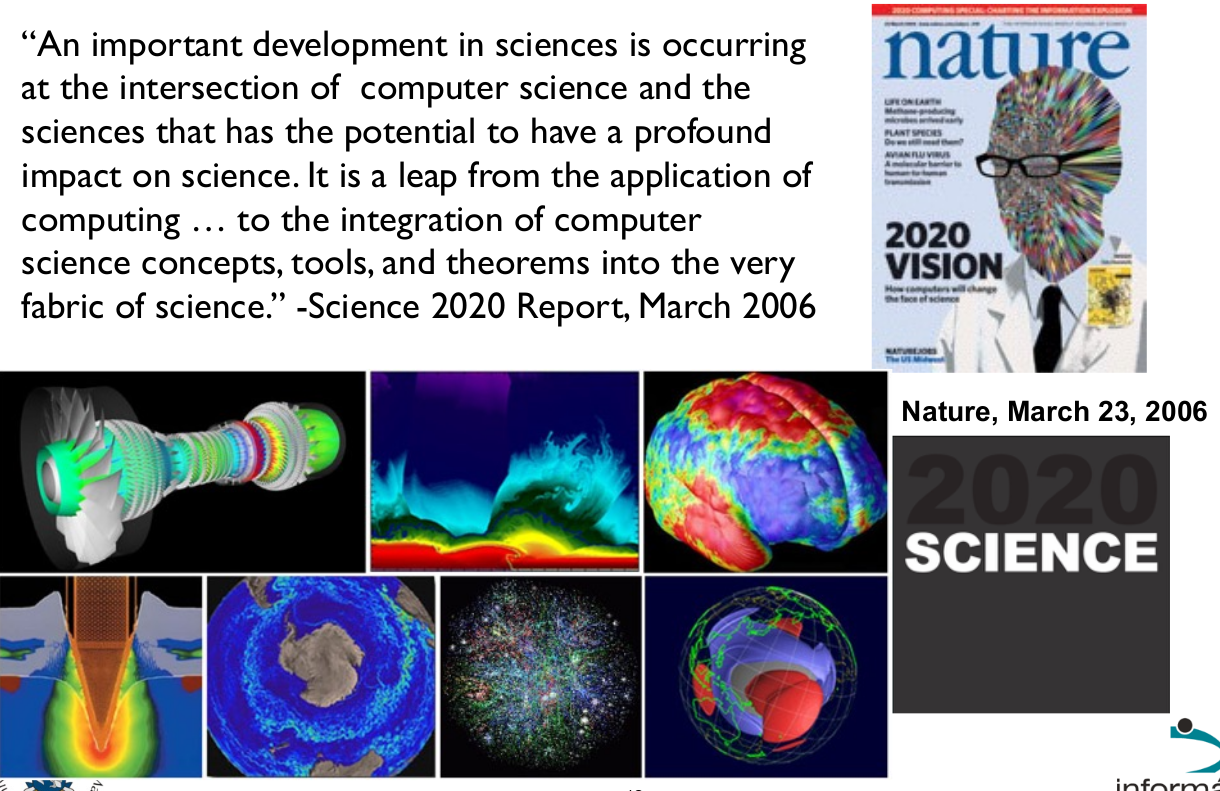
\includegraphics[width=0.8\textwidth]{comp.png}
  \end{center}
\end{frame}
%------------------------------------------------------------------------------
\begin{frame}
  \frametitle{Computação Científica}
    \begin{itemize}
      \item Simulação - chamado \textbf{Terceiro Pilar da Ciência}
      \item Método tradicional da Ciência e Engenharia
            \begin{itemize}
                \item Cria a teoria ou projeto
                \item Faz experimentos ou constrói sistemas
            \end{itemize}
        \item Limitações
            \begin{itemize}
                \item Muito difícil -- construir grandes túneis de vento
                \item Muito caro -- construir um jato que projeta pessoas
                \item Perigoso -- armas, medicamentos, experiemntos climatológicos
            \end{itemize}
    \end{itemize}
\end{frame}
%------------------------------------------------------------------------------
\begin{frame}
  \frametitle{Computação Científica}
    \begin{itemize}
      \item \textbf{Paradigma da Computação Científica}
      \item Computadores para simular e analisar um fenômeno 
      \item Baseado no conhecimento de leis físicas e métodos numéricos eficientes
      \item Analisar resultados de simulações resulta em ferramentas e métodos além do que é possível
    \end{itemize}
  \begin{center}
    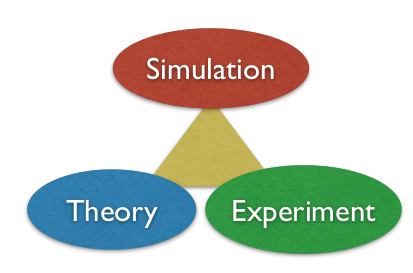
\includegraphics[width=0.5\textwidth]{tripe.png}
  \end{center}
\end{frame}
%------------------------------------------------------------------------------
%\includeslides{2-3}{palestra-pet-si-jun2015.pdf}
{\setbeamercolor{background canvas}{bg=}
\includepdf[pages=52-64,%
    %pagecommand={\begin{frame}[default]{}\end{frame}},
    pagecommand={},
%    #4,%
turn=false,noautoscale=false,column=false,columnstrict=false,openright=false,frame=false]{palestra-pet-si-jun2015.pdf}%
}
%------------------------------------------------------------------------------
%%%%%%%%%%%%%%%%%%%%%%%%%%%%%%%%%%%%%%%%%%%%%%%%%%%%%%%%%%%%%%%%%%%%%%%%%%%%%%
\section{Programação Paralela}
%%%%%%%%%%%%%%%%%%%%%%%%%%%%%%%%%%%%%%%%%%%%%%%%%%%%%%%%%%%%%%%%%%%%%%%%%%%%%%%
{\setbeamercolor{background canvas}{bg=}
\includepdf[pages=36-47,%
    %pagecommand={\begin{frame}[default]{}\end{frame}},
    pagecommand={},
%    #4,%
turn=false,noautoscale=false,column=false,columnstrict=false,openright=false,frame=false]{palestra-pet-si-jun2015.pdf}%
}
\begin{frame}[plain]{}
  \begin{center}
    \vspace{2cm}
    \Large{https://joao-ufsm.github.io/par2023a/}
    
    \vspace{1cm}
    
\includegraphics[width=2cm]{logo_ufsm}
    \hspace{0.5cm}
    
\includegraphics[width=2cm]{logo_inf}
  \end{center}
\end{frame}
%------------------------------------------------------------------------------

\end{document}
